%
% quotientv.tex
%
% (c) 2021 Prof Dr Andreas Müller, OST Ostschweizer Fachhochschule
%
\bgroup
\definecolor{darkred}{rgb}{0.7,0,0}
\definecolor{darkgreen}{rgb}{0,0.6,0}
\begin{frame}[t]
\frametitle{Quotient}
\vspace{-18pt}
\begin{columns}[t,onlytextwidth]
\begin{column}{0.33\textwidth}
\begin{block}{Repräsentanten}
Jeder Unterraum $W\subset V$ mit 
$W\cap U = \{0\}$
kann als Menge von Repräsentanten
für
\begin{align*}
V/U
&=
\{v+U\;|\;v \in V\}
\\
&\simeq W
\end{align*}
dienen.
\end{block}
\uncover<3->{%
\begin{block}{Orthogonalraum}
Mit Skalarprodukt ist
$W=U^\perp$ eine bevorzugte Wahl
\end{block}}
\end{column}
\begin{column}{0.66\textwidth}
\begin{center}
\begin{tikzpicture}[>=latex,thick]
\only<1>{
	\node at (0,0)
	{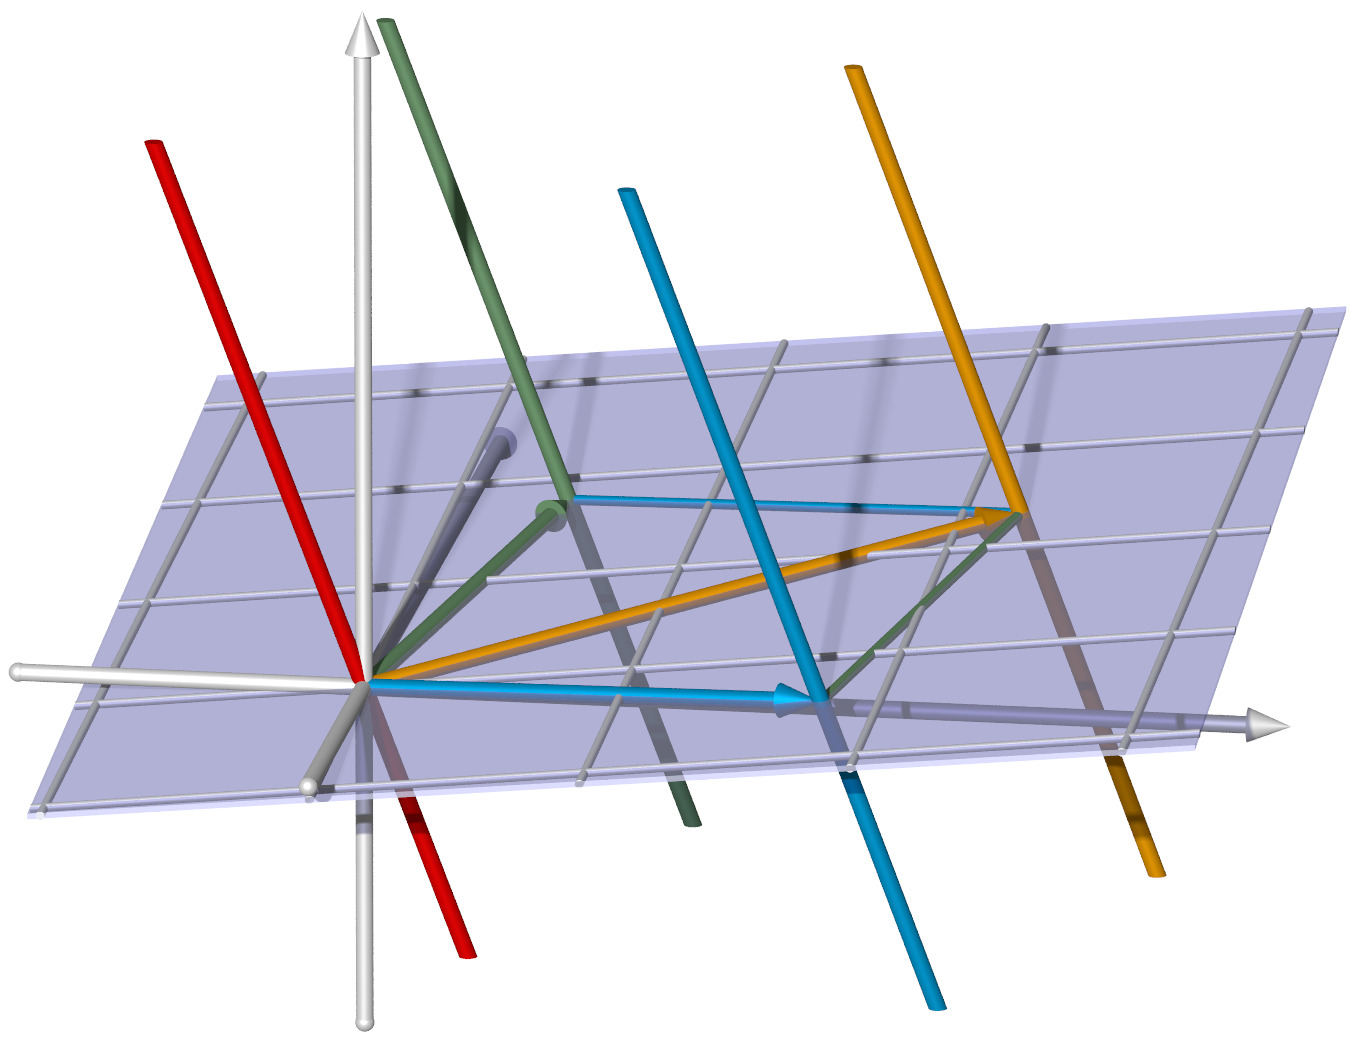
\includegraphics[width=8.5cm]{../slides/2/images/quotient1.jpg}};
	\node[color=darkgreen] at (-0.5,0.3) {$v$};
	\node[color=blue] at (0.7,-1.4) {$w$};
	\node[color=orange] at (2.7,0.1) {$v+w$};
	\fill[color=white,opacity=0.5] (3.7,1.0) circle[radius=0.25];
	\node at (3.7,1.0) {$W$};
}
\only<2->{
	\node at (0,0)
	{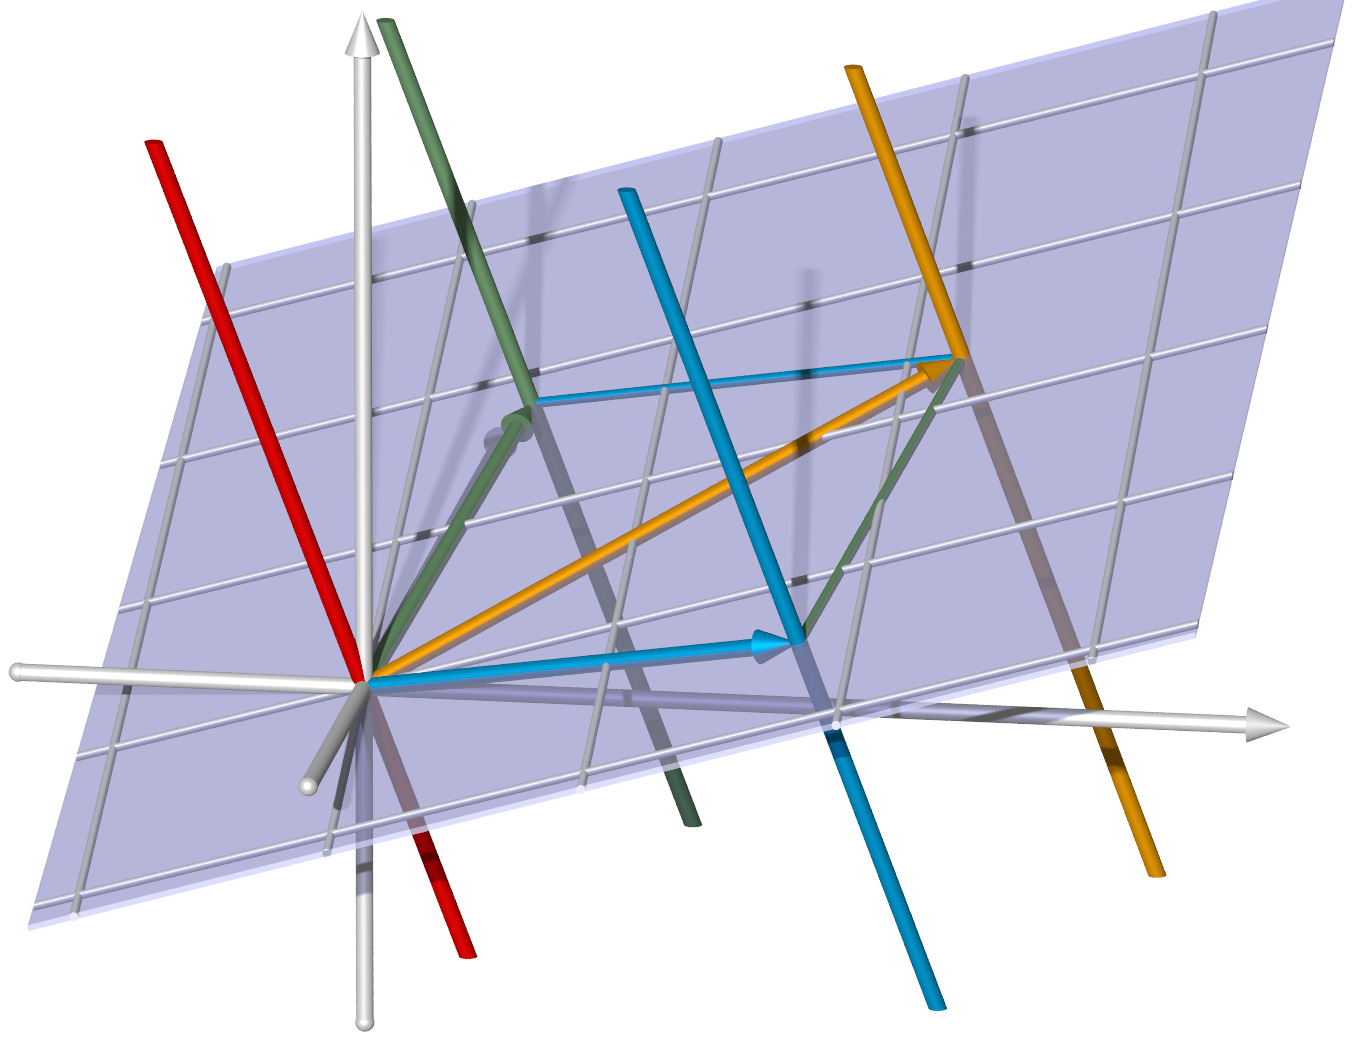
\includegraphics[width=8.5cm]{../slides/2/images/quotient2.jpg}};
	\node[color=darkgreen] at (-0.75,0.95) {$v$};
	\node[color=blue] at (0.6,-1.05) {$w$};
	\node[color=orange] at (2.36,1.05) {$v+w$};
	\fill[color=white,opacity=0.5] (3.7,2.9) circle[radius=0.25];
	\node at (3.7,2.9) {$W$};
}
\node[color=darkred] at (-3.3,2.6) {$U$};
\node[color=darkred] at (-2.25,-1.0) {$0$};
\end{tikzpicture}
\end{center}
\end{column}
\end{columns}
\end{frame}
\egroup
